\subsection[\englishfont 2.4 超视距碰撞预警原型系统设计及实现]{2.4 超视距碰撞预警原型系统设计及实现}

\begin{frame}
\frametitle{\englishfont 研究贡献}
\newBackground
\begin{center}
\begin{textblock*}{\textwidth}(-2cm,1.8cm)
\begin{spacing}{0}
  \small \englishfont \colorbox{cqublue}{\color{white}{原型系统的设计和实现是针对VCPS必要的{\color{yellow}{验证手段}}}}
\end{spacing}
\end{textblock*}
\end{center}

\begin{center}
\begin{textblock*}{\textwidth}(-1.8cm,2.8cm)
\begin{minipage}[t]{0.7\textwidth}
\begin{itemize}[itemsep=0.2\baselineskip] \englishfont 
	\item[\ding{111}] {{\color{cqublue}{\textbf{算法}}}:基于VCPS优化的碰撞预警} 
	\begin{itemize}[itemsep=0.2\baselineskip]
	\begin{small}
		\item[\ding{226}] 基于稳定分布的V2I应用层传输时延拟合模型
		\item[\ding{226}] 基于车辆轨迹和历史信息的丢包检测机制
	\end{small}
	\end{itemize}
	\item[\ding{111}]  {{\color{cqublue}{\textbf{系统}}}:超视距碰撞预警{\color{red}{原型系统}}}
	\begin{itemize}
	\begin{small}
		\item[\ding{226}] 基于C-V2X设备的硬件在环试验平台
		\item[\ding{226}] 原型系统实现
	\end{small}
	\end{itemize}
\end{itemize}
\end{minipage}
\end{textblock*}
\end{center}

\begin{center}
\begin{textblock*}{\textwidth}(-2cm,6.5cm)
\fbox{\begin{minipage}[t]{0.65\textwidth}\englishfont \tiny [6] \underline{\textcolor{cqublue}{XU X}}, LIU K, XIAO K, et al. \textcolor{cqublue}{Vehicular fog computing enabled real-time collision warning via trajectory calibration}[J]. Mobile Networks and Applications (\textcolor{red}{MONET}), 2020, 25(6): 2482-2494. 影响因子: 3.077(2021), 2.92(5年) (中科院SCI 3区)
\end{minipage}}
\fbox{\begin{minipage}[t]{0.65\textwidth}\englishfont \tiny [7] \underline{\textcolor{cqublue}{XU X}}, LIU K, XIAO K, et al. \textcolor{cqublue}{Design and implementation of a fog computing based collision warning system in VANETs}[C]. IEEE ISPCE-CN, 2018. (最佳论文奖)
\end{minipage}}
\end{textblock*}
\end{center}

\begin{center}
\begin{textblock*}{\textwidth}(6cm,1.8cm)
\begin{figure}
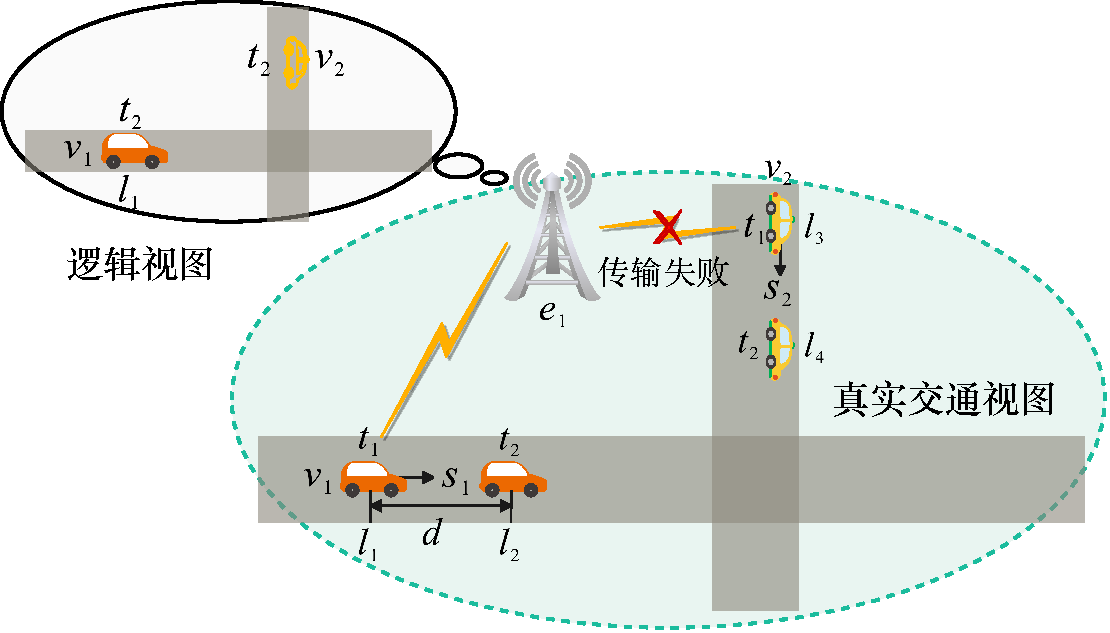
\includegraphics[width=0.4\textwidth]{fig/Fig5-1-example.pdf}
\end{figure}
\begin{figure}
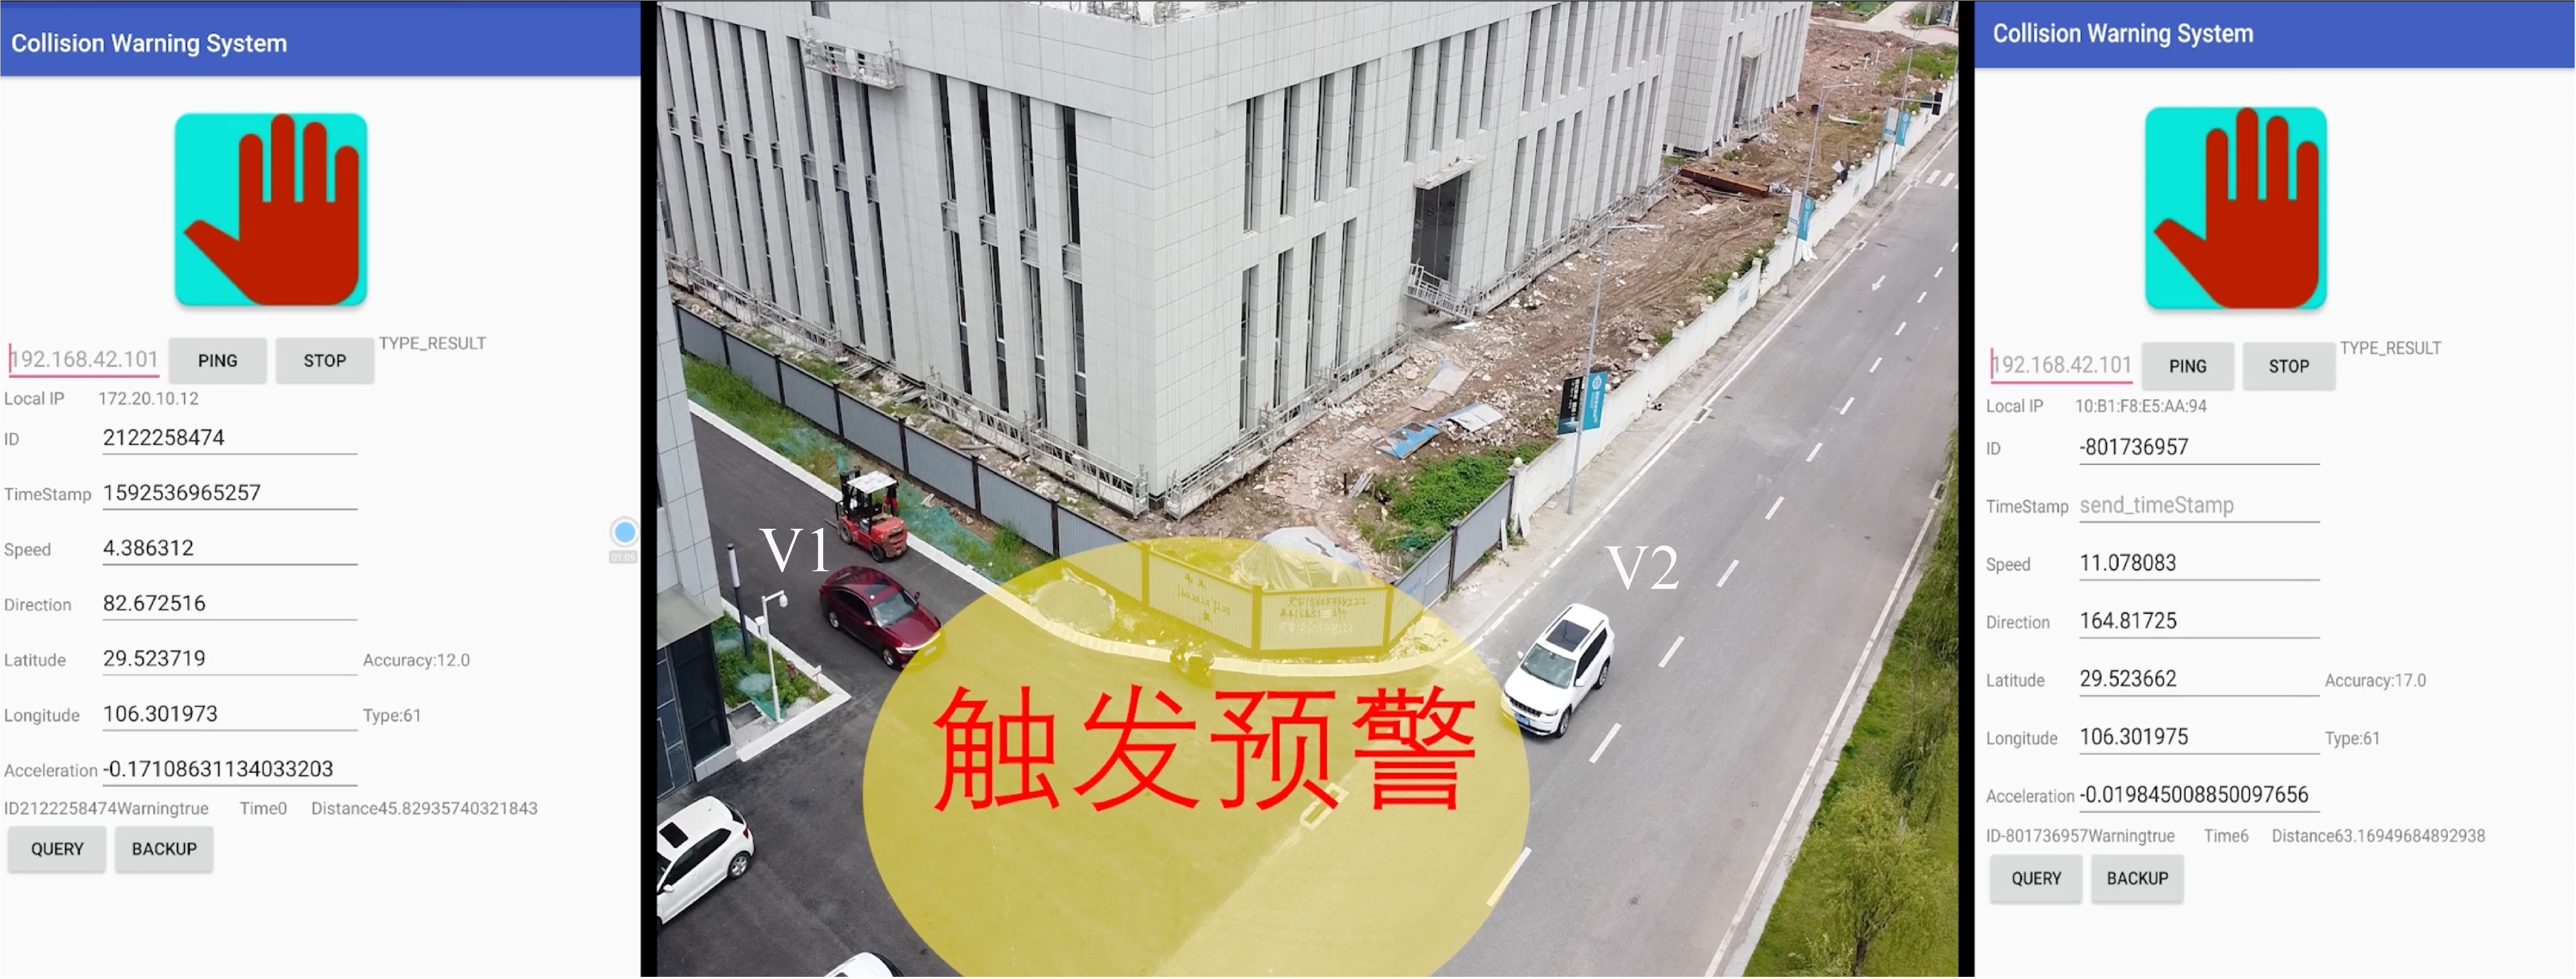
\includegraphics[width=0.4\textwidth]{fig/Fig5-12-2.pdf}
\end{figure}
\end{textblock*}
\end{center}
\end{frame}

\begin{frame}
\frametitle{\englishfont \underline{算法}:流程}
\newBackground

\begin{center}
\begin{textblock*}{1\textwidth}(0.5cm,1.8cm)
\begin{itemize}[itemsep=0.2\baselineskip] \englishfont
\item[\ding{111}] {\color{cqublue}{车辆状态更新}}
	\begin{itemize}[itemsep=0.2\baselineskip]
	\begin{small}
		\item[\ding{226}] 基于V2I传输时延拟合模型估计传输时延
		\item[\ding{226}] 根据车辆速度和加速度更新其实时状态
	\end{small}
	\end{itemize}	
\item[\ding{111}] {\color{cqublue}{丢包检测}}
	\begin{itemize}[itemsep=0.2\baselineskip]
	\begin{small}
		\item[\ding{226}] 根据历史位置判断车辆是否在通信范围内
		\item[\ding{226}] 在通信范围内却未收到数据包,则认为已丢失
		\item[\ding{226}] 丢失的数据包使用历史记录更新它们的状态
	\end{small}
	\end{itemize}
	\item[\ding{111}] {\color{cqublue}{轨迹预测}}
	\begin{itemize}[itemsep=0.2\baselineskip]
	\begin{small}
		\item[\ding{226}] 基于修正的视图预测所有车辆未来的轨迹
	\end{small}
	\end{itemize}
	\item[\ding{111}] {\color{cqublue}{碰撞预警}}
	\begin{itemize}[itemsep=0.2\baselineskip]
	\begin{small}
		\item[\ding{226}] 计算每对车辆的车头时距
		\item[\ding{226}]通过车头时距阈值来检测潜在碰撞
	\end{small}
	\end{itemize}
\end{itemize}
\end{textblock*}
\end{center}

\begin{center}
\begin{textblock*}{\textwidth}(5.2cm,2.6cm)
\begin{figure}
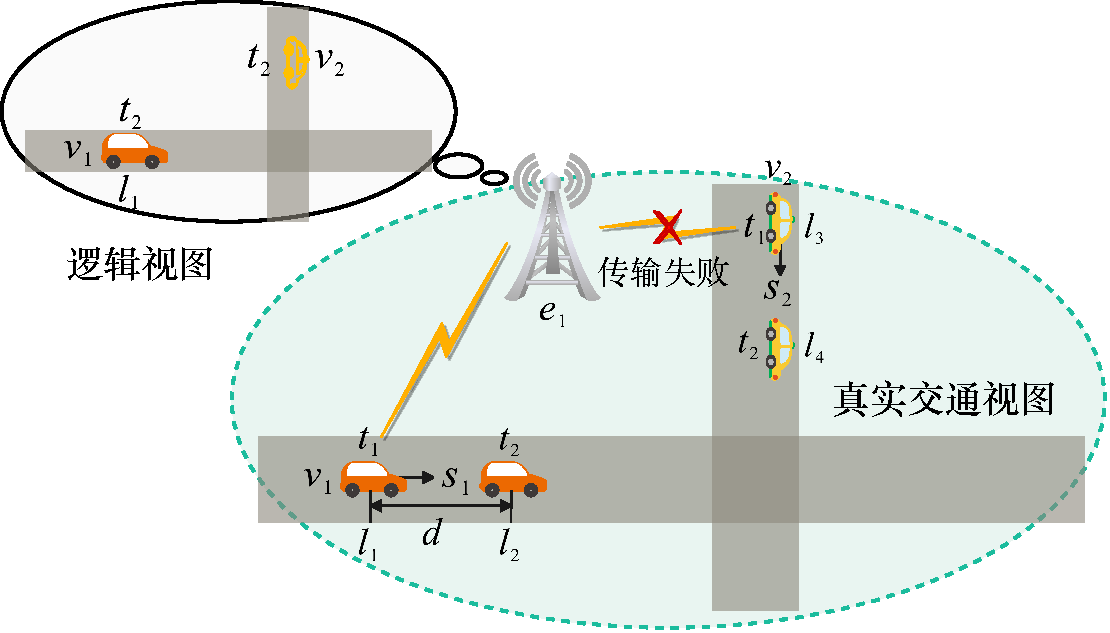
\includegraphics[width=0.45\textwidth]{fig/Fig5-1-example.pdf}
\end{figure}
\end{textblock*}
\end{center}

\end{frame}

\begin{frame}
\frametitle{\englishfont \underline{算法}:V2I应用层时延拟合模型}
\newBackground

\begin{center}
\begin{textblock*}{0.7\textwidth}(0cm,4.2cm)
	\scriptsize
	\begin{numcases}{E \exp (i t X)=}
\exp \left\{-\sigma^{\alpha}|t|^{\alpha}[1-i \beta \tan (\alpha \pi / 2) \operatorname{sgn}(t)]+i \mu t\right\}, &$\alpha \neq 1$ \notag \\
\exp \{-\sigma|t[1+i \beta(2 / \pi) \operatorname{sgn}(t) \ln (|t|)]+i \mu t\},  &$\alpha=1$ \notag
\end{numcases}
\end{textblock*}
\end{center}

\begin{center}
\begin{textblock*}{0.7\textwidth}(0.5cm,1.8cm)
\begin{itemize}[itemsep=0.2\baselineskip] \englishfont 
	\item[\ding{111}]  {\color{cqublue}{数据}}
	\begin{itemize}[itemsep=0.2\baselineskip]
	\begin{small}
		\item[\ding{226}] 现场测试得到传输时延数据
		\item[\ding{226}] 分布不服从高斯分布
	\end{small} 
	\end{itemize}
	\item[\ding{111}]  {\color{cqublue}{稳定分布}}
	\begin{itemize}[itemsep=0.2\baselineskip]
	\begin{small}
		\item[\ding{226}] 适用于对非高斯过程进行估计
		\item
		\item
	\end{small} 
	\end{itemize}
	\item[\ding{111}]  {\color{cqublue}{拟合结果}}
	\begin{itemize}[itemsep=0.2\baselineskip]
	\begin{small}
	\item[\ding{226}] 几乎是对称的 ($\alpha = 1.77395$)
	\item[\ding{226}] 围绕均值 ($\mu = 72.7343$)
	\item[\ding{226}] 分布具有左偏度 ($\beta = 1$)
	\item[\ding{226}] 与均值的离散程度较大 ($\sigma = 13.3685$)
	\end{small} 
	\end{itemize}
\end{itemize}
\end{textblock*}
\end{center}

\begin{center}
\begin{textblock*}{\textwidth}(5.8cm,2.6cm)
\begin{figure}
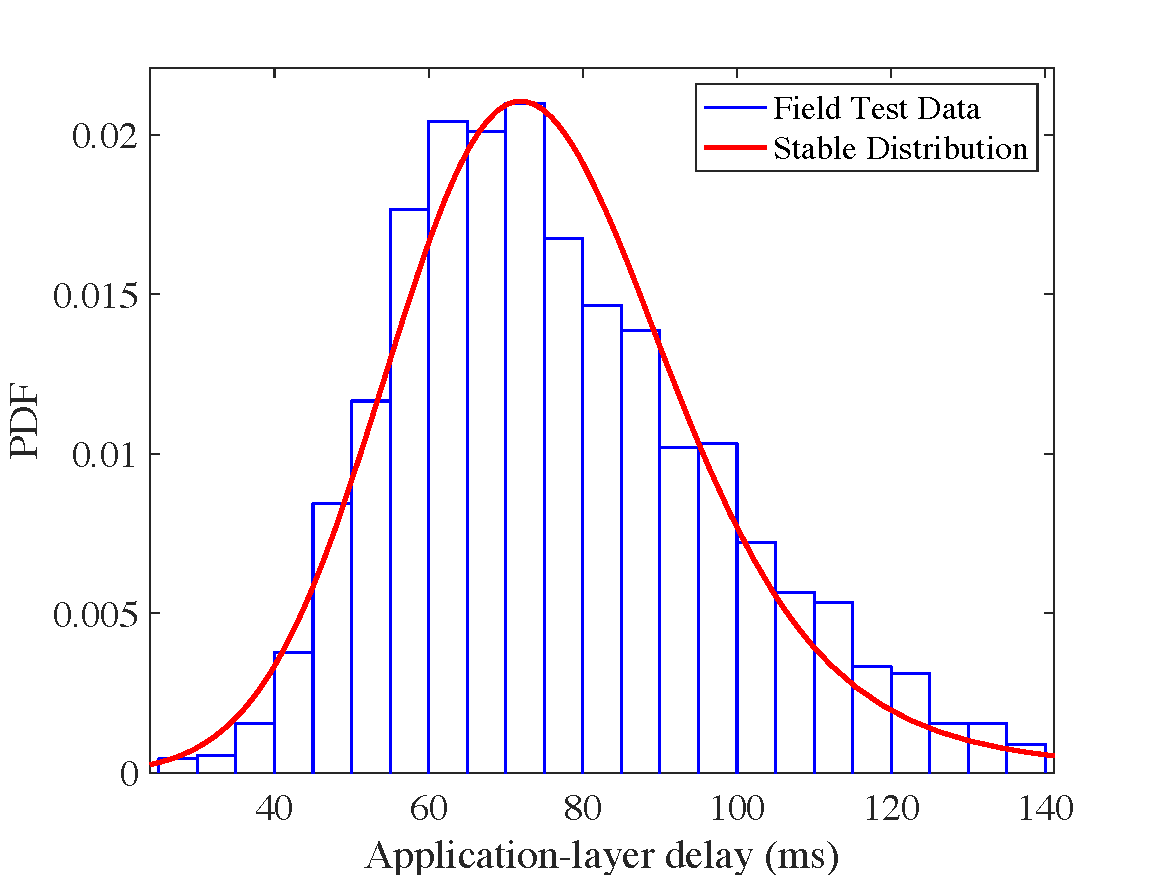
\includegraphics[width=0.43\textwidth]{fig/Fig5-3-delay-fitting.pdf}
\end{figure}
\end{textblock*}
\end{center}

\end{frame}


\begin{frame}
\frametitle{\englishfont \underline{系统}:硬件在环平台框架}
\newBackground
\begin{center}
\begin{textblock*}{\textwidth}(5.3cm,2.5cm)
\begin{figure}
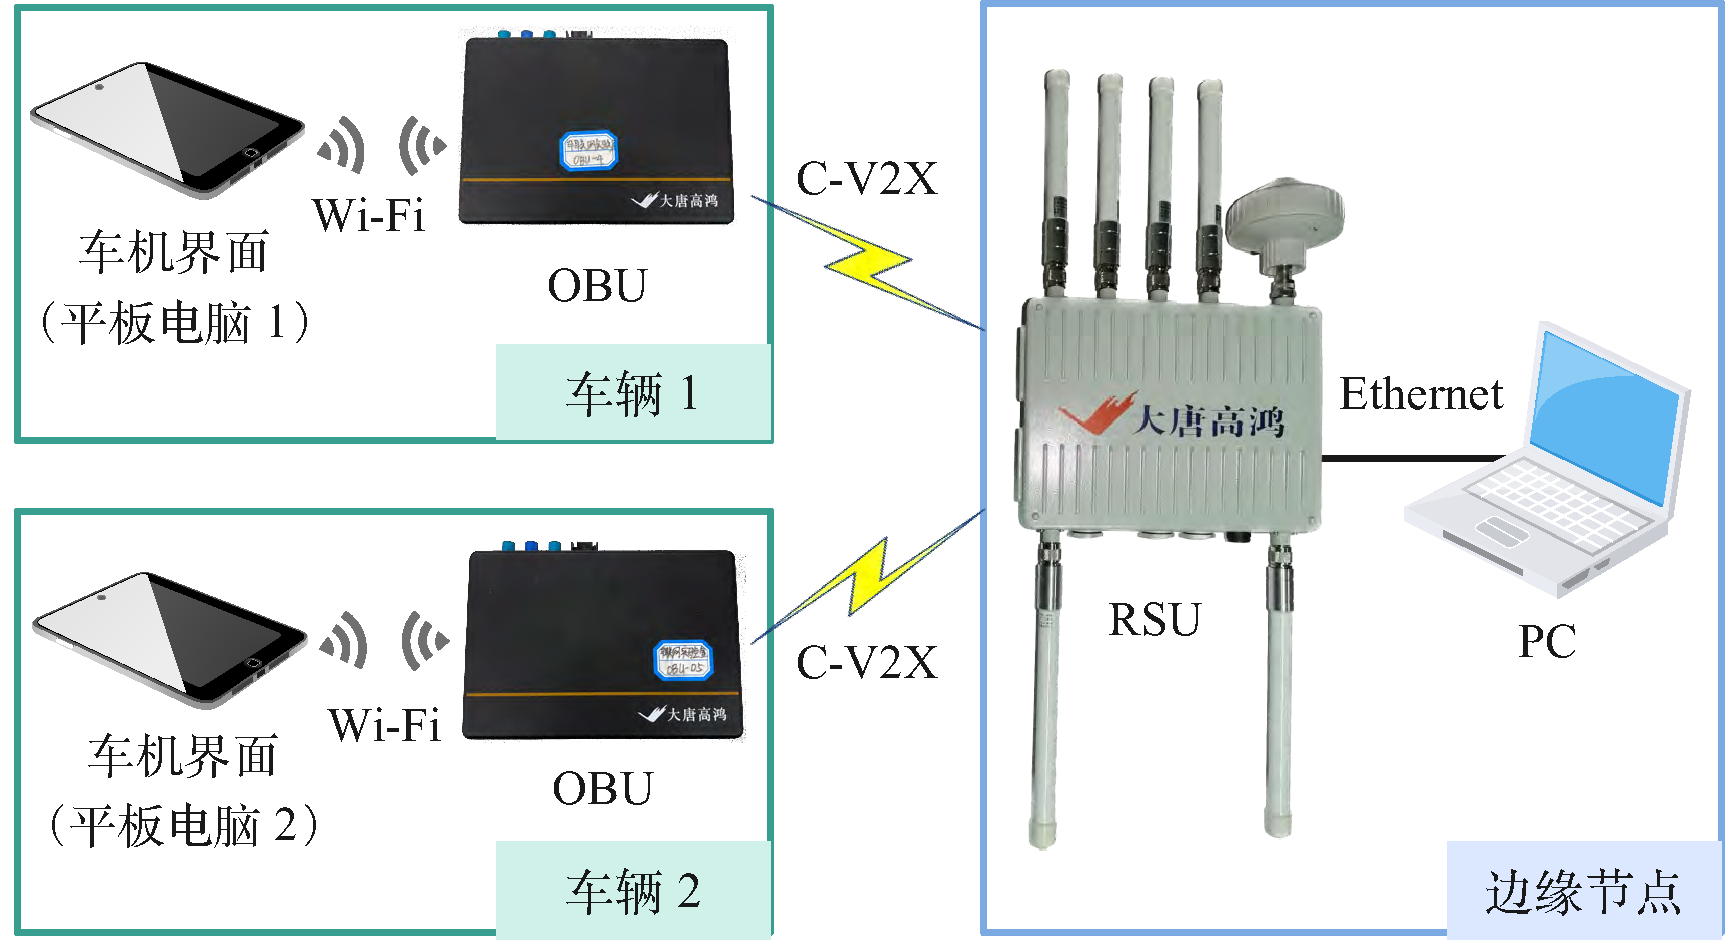
\includegraphics[width=0.5\textwidth]{fig/Fig5-8-hardware-in-the-loop-architecture.pdf}
\end{figure}
\end{textblock*}
\end{center}

\begin{center}
\begin{textblock*}{0.55\textwidth}(0.5cm,1.8cm)
\begin{itemize}[itemsep=0.2\baselineskip] \englishfont 
	\item[\ding{111}] {\color{cqublue}{硬件设备}}
	\begin{itemize}[itemsep=0.2\baselineskip]
	\begin{small}
		\item[\ding{226}] C-V2X 车载终端 (OBU)和路侧设备 (RSU)
		\item[\ding{226}] LTE-V2X PC5 和 5G UU 双模通信能力		
		\item[\ding{226}] 具有 GNSS 天线,可接收 GPS 卫星信号
	\end{small}
	\end{itemize}
	\item[\ding{111}] {\color{cqublue}{车端}}
	\begin{itemize}[itemsep=0.2\baselineskip]
	\begin{small}
		\item[\ding{226}] OBU 与平板电脑通过Wi-Fi 相互通信
		\item[\ding{226}] 平板电脑可作为车机界面进行碰撞预警消息的可视化
	\end{small}
	\end{itemize}
	\item[\ding{111}] {\color{cqublue}{边缘端}}
	\begin{itemize}[itemsep=0.2\baselineskip]
	\begin{small}
		\item[\ding{226}] PC 通过以太网与 RSU 相连
		\item[\ding{226}] PC 作为计算单元提供服务
	\end{small}
	\end{itemize}
\end{itemize}
\end{textblock*}
\end{center}
\end{frame}

\begin{frame}{基于 C-V2X 的硬件在环试验平台}
\newBackground
\begin{center}
\begin{textblock*}{\textwidth}(1cm,1.8cm)
\begin{figure}
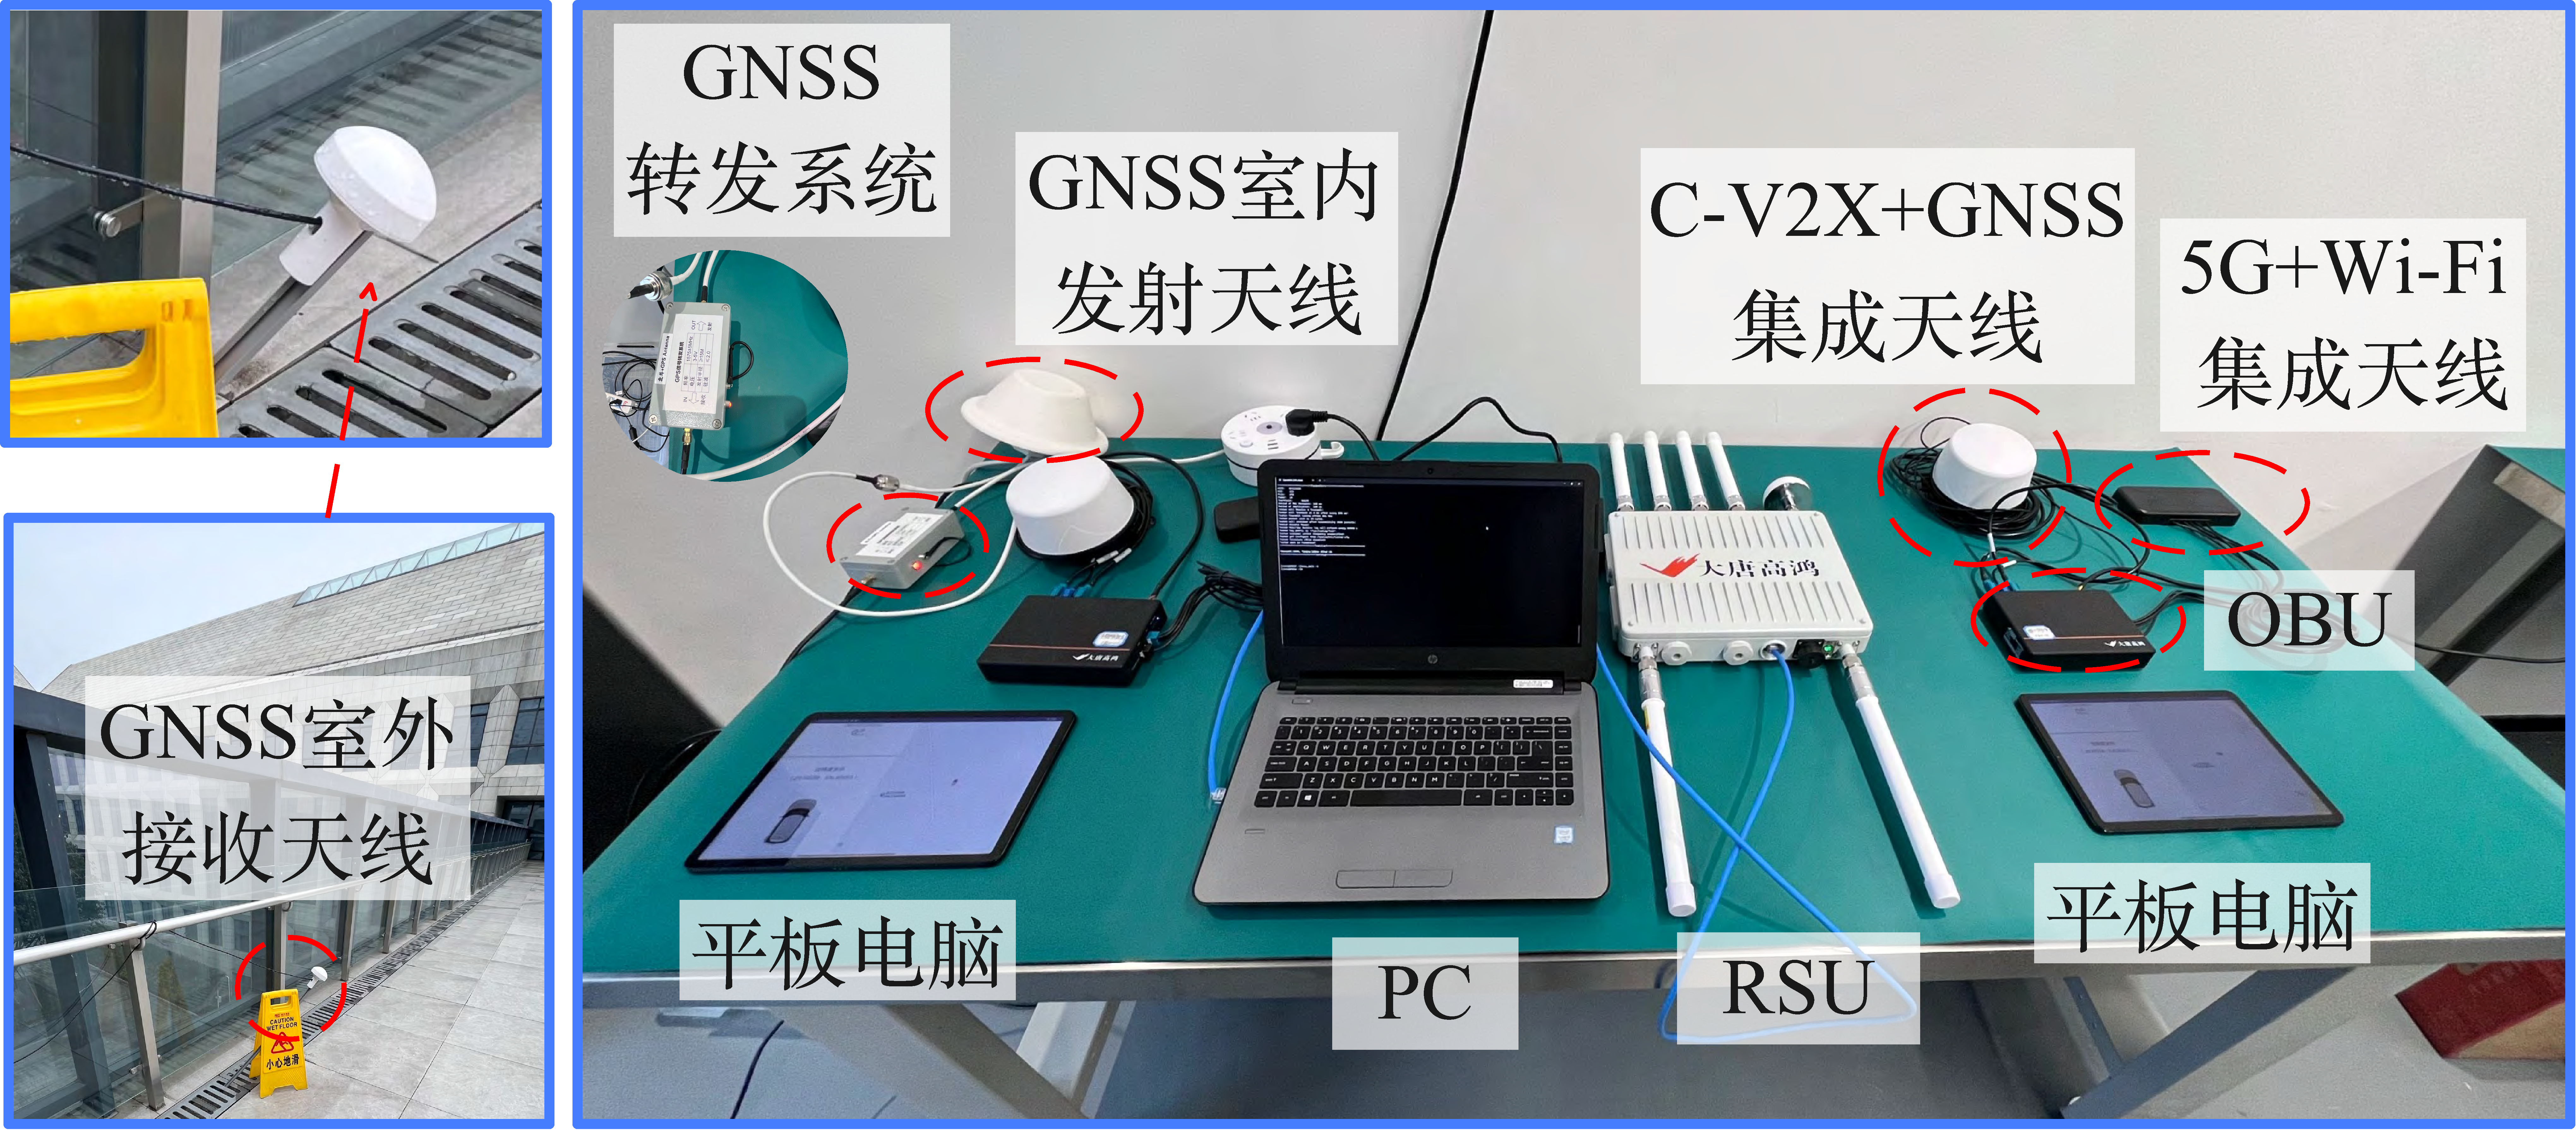
\includegraphics[width=1\textwidth]{fig/Fig5-9-C-V2X-hardware-in-loop.pdf}
\end{figure}
\end{textblock*}
\end{center}
\end{frame}

\begin{frame}
\frametitle{\englishfont \underline{系统}:C-V2X 端到端时延}
\newBackground
\begin{center}
\begin{textblock*}{\textwidth}(5.2cm,2.2cm)
\begin{figure}
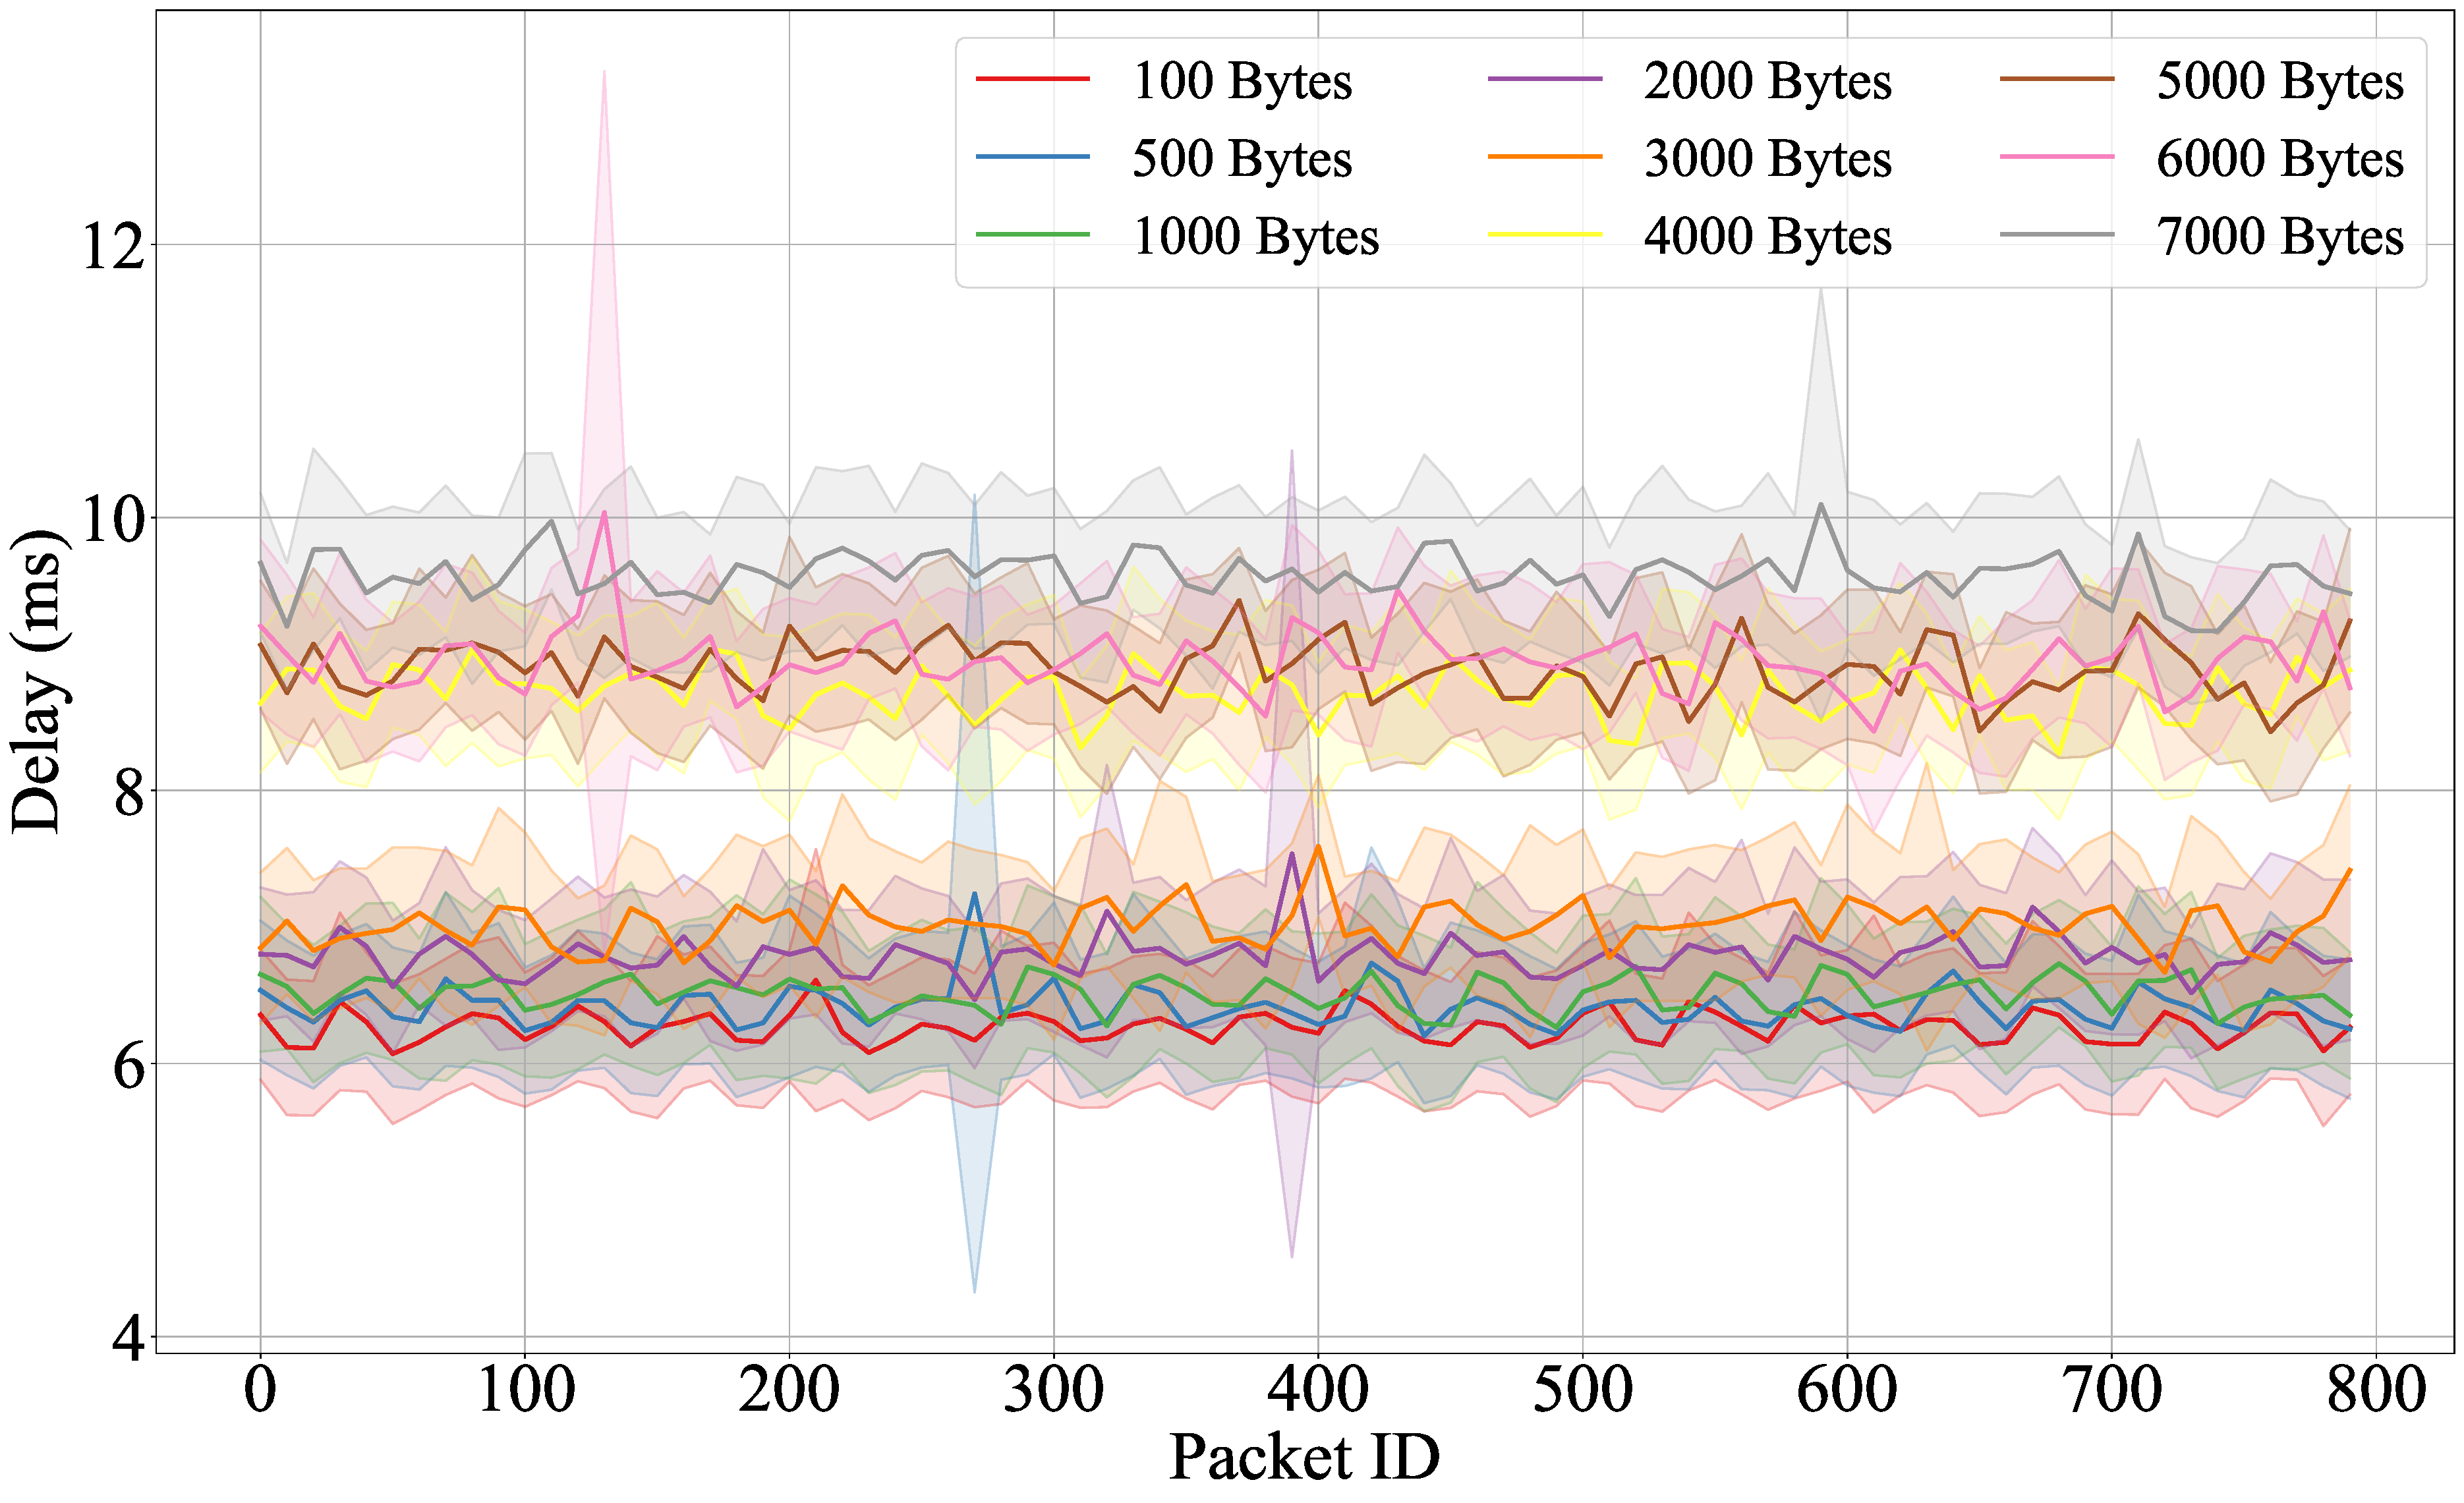
\includegraphics[width=0.5\textwidth]{fig/Fig5-10-delays.pdf}
\end{figure}
\end{textblock*}
\end{center}

\begin{center}
\begin{textblock*}{0.55\textwidth}(0.5cm,2.3cm)
\begin{itemize}[itemsep=0.2\baselineskip] \englishfont 
	\item[\ding{111}] {\color{cqublue}{数据包设置}}
	\begin{itemize}[itemsep=0.2\baselineskip]
	\begin{small}
		\item[\ding{226}] 以10 Hz的频率分别发送1000个数据包
		\item[\ding{226}] 大小从100 Bytes增加至7000 Bytes	
	\end{small}
	\end{itemize}
	\item[\ding{111}] {\color{cqublue}{时延结果分析}}
	\begin{itemize}[itemsep=0.2\baselineskip]
	\begin{small}
		\item[\ding{226}] 最小数据包 (100 Bytes)平均时延最短 (6.271 ms)
		\item[\ding{226}] 最大数据包 (7000 Bytes)平均时延最长 (9.570 ms)
	\end{small}
	\end{itemize}
\end{itemize}
\end{textblock*}
\end{center}

\end{frame}